% Poster (French): NISAR vs Sentinel-1 over forests in France. Build: cd poster && lualatex poster_forets_fr.tex
% Figures: python poster/poster_figures.py (from the repository root), read from the result tables.
\documentclass[20pt,a0paper,portrait,margin=0mm,innermargin=18mm,blockverticalspace=14mm,colspace=16mm,subcolspace=8mm]{tikzposter}
\usepackage[french]{babel}
\usepackage{fontspec}
\setmainfont{TeX Gyre Heros}
\usepackage{graphicx,booktabs,xcolor,amsmath,enumitem,tabularx}
\usetikzlibrary{positioning,arrows.meta,fit,calc}
\usepackage[hidelinks]{hyperref}
\definecolor{accent}{HTML}{2E7D32}
\definecolor{nuit}{HTML}{12304F}
\definecolor{bandeL}{HTML}{1F5FAE}
\definecolor{bandeC}{HTML}{D4541F}
\definecolor{fond}{HTML}{F5F8FB}
\definecolor{gris}{HTML}{555555}
\usetheme{Simple}
\colorlet{backgroundcolor}{white}
\colorlet{framecolor}{white}
\colorlet{blocktitlebgcolor}{nuit}
\colorlet{blocktitlefgcolor}{white}
\colorlet{blockbodybgcolor}{fond}
\colorlet{blockbodyfgcolor}{black}
\colorlet{titlebgcolor}{white}
\colorlet{titlefgcolor}{nuit}
\defineblockstyle{Plat}{titlewidthscale=1, bodywidthscale=1, titleleft, titleoffsetx=0pt, titleoffsety=0pt,
  bodyoffsetx=0mm, bodyoffsety=12mm, bodyverticalshift=12mm, roundedcorners=6, linewidth=0pt,
  titleinnersep=9mm, bodyinnersep=11mm}{
  \draw[color=framecolor, fill=blockbodybgcolor, rounded corners=\blockroundedcorners] (blockbody.south west) rectangle (blockbody.north east);
  \ifBlockHasTitle
    \draw[color=framecolor, fill=blocktitlebgcolor, rounded corners=\blockroundedcorners] (blocktitle.south west) rectangle (blocktitle.north east);
  \fi}
\useblockstyle{Plat}
\setlist{leftmargin=1.1em,itemsep=4pt,topsep=4pt}
\newcommand{\Lb}[1]{\textcolor{bandeL}{\textbf{#1}}}
\newcommand{\Cb}[1]{\textcolor{bandeC}{\textbf{#1}}}
\newcommand{\fig}[2][1]{\begin{center}\includegraphics[width=#1\linewidth]{#2}\end{center}}
\newcounter{numfig}\newcounter{numtab}
\newcommand{\figcap}[1]{\stepcounter{numfig}{\small\textbf{Figure \thenumfig.} #1\par}\vspace{2mm}}
\newcommand{\tabcap}[1]{\stepcounter{numtab}{\small\textbf{Tableau \thenumtab.} #1\par}\vspace{1mm}}
\newcommand{\sous}[1]{\par\vspace{3mm}{\color{nuit}\large\bfseries #1\par}\vspace{1mm}}
\newcommand{\cle}[1]{\vspace{4mm}\colorbox{accent!12}{\parbox{0.97\linewidth}{\vspace{3mm}#1\vspace{3mm}}}\vspace{2mm}}

\settitle{
\begin{minipage}[c]{\linewidth}\centering
{\color{nuit}\fontsize{66}{78}\selectfont\bfseries Les forêts françaises vues par NISAR\\[5mm]
\fontsize{50}{60}\selectfont bande L contre bande C pour les coupes rases et un glissement sous forêt\par}
\vspace{9mm}
{\fontsize{40}{48}\selectfont\color{black}\textbf{Mamadou Galy DIALLO}\par}
\vspace{3mm}
{\fontsize{30}{38}\selectfont\color{gris}galy.quantum@gmail.com\par}
\end{minipage}
\vspace{8mm}
{\color{accent}\rule{\linewidth}{5mm}}
}

\tikzposterlatexaffectionproofoff
\graphicspath{{figures/}}
\begin{document}
\maketitle[width=0.95\paperwidth, titletotopverticalspace=12mm, titletoblockverticalspace=10mm]

\begin{columns}
% ===================================================================== colonne gauche
\column{0.5}

\block{1. Introduction}{
Détecter les coupes rases et suivre les glissements sous forêt sont deux besoins de la gestion forestière
et de la prévention des risques. L'optique, référence pour les coupes rases [3], dépend des nuages. Le radar en \Cb{bande C} de Sentinel-1 (5,6 cm) [2], gratuit
et acquis tous les 6 à 12 jours, est surtout sensible aux feuilles et aux petites branches : sous la forêt, sa
cohérence interférométrique chute en quelques jours [4]. La \Lb{bande L} (24 cm) pénètre davantage le houppier
et interagit avec les troncs et les grosses branches [5]. Depuis 2025, \textbf{NISAR} (NASA--ISRO) [1] fournit une série
en bande L gratuite tous les \textbf{12 jours}. \textbf{Ainsi, cette étude compare la bande L (NISAR) et la bande C (Sentinel-1)
sur trois cas forestiers français, avec les premières données de juin à novembre 2026.}
\sous{Objectif}
Mesurer, pour une coupe rase récente (Vosges) puis pour sept coupes vérifiées (Morvan), laquelle des deux
bandes sépare le mieux la coupe de la forêt intacte, en rétrodiffusion et en cohérence ; puis vérifier, sur
le glissement de Séchilienne, si la phase interférométrique reste exploitable sous la forêt.
}

\block{2. Sites et données}{
\begin{minipage}[c]{0.38\linewidth}
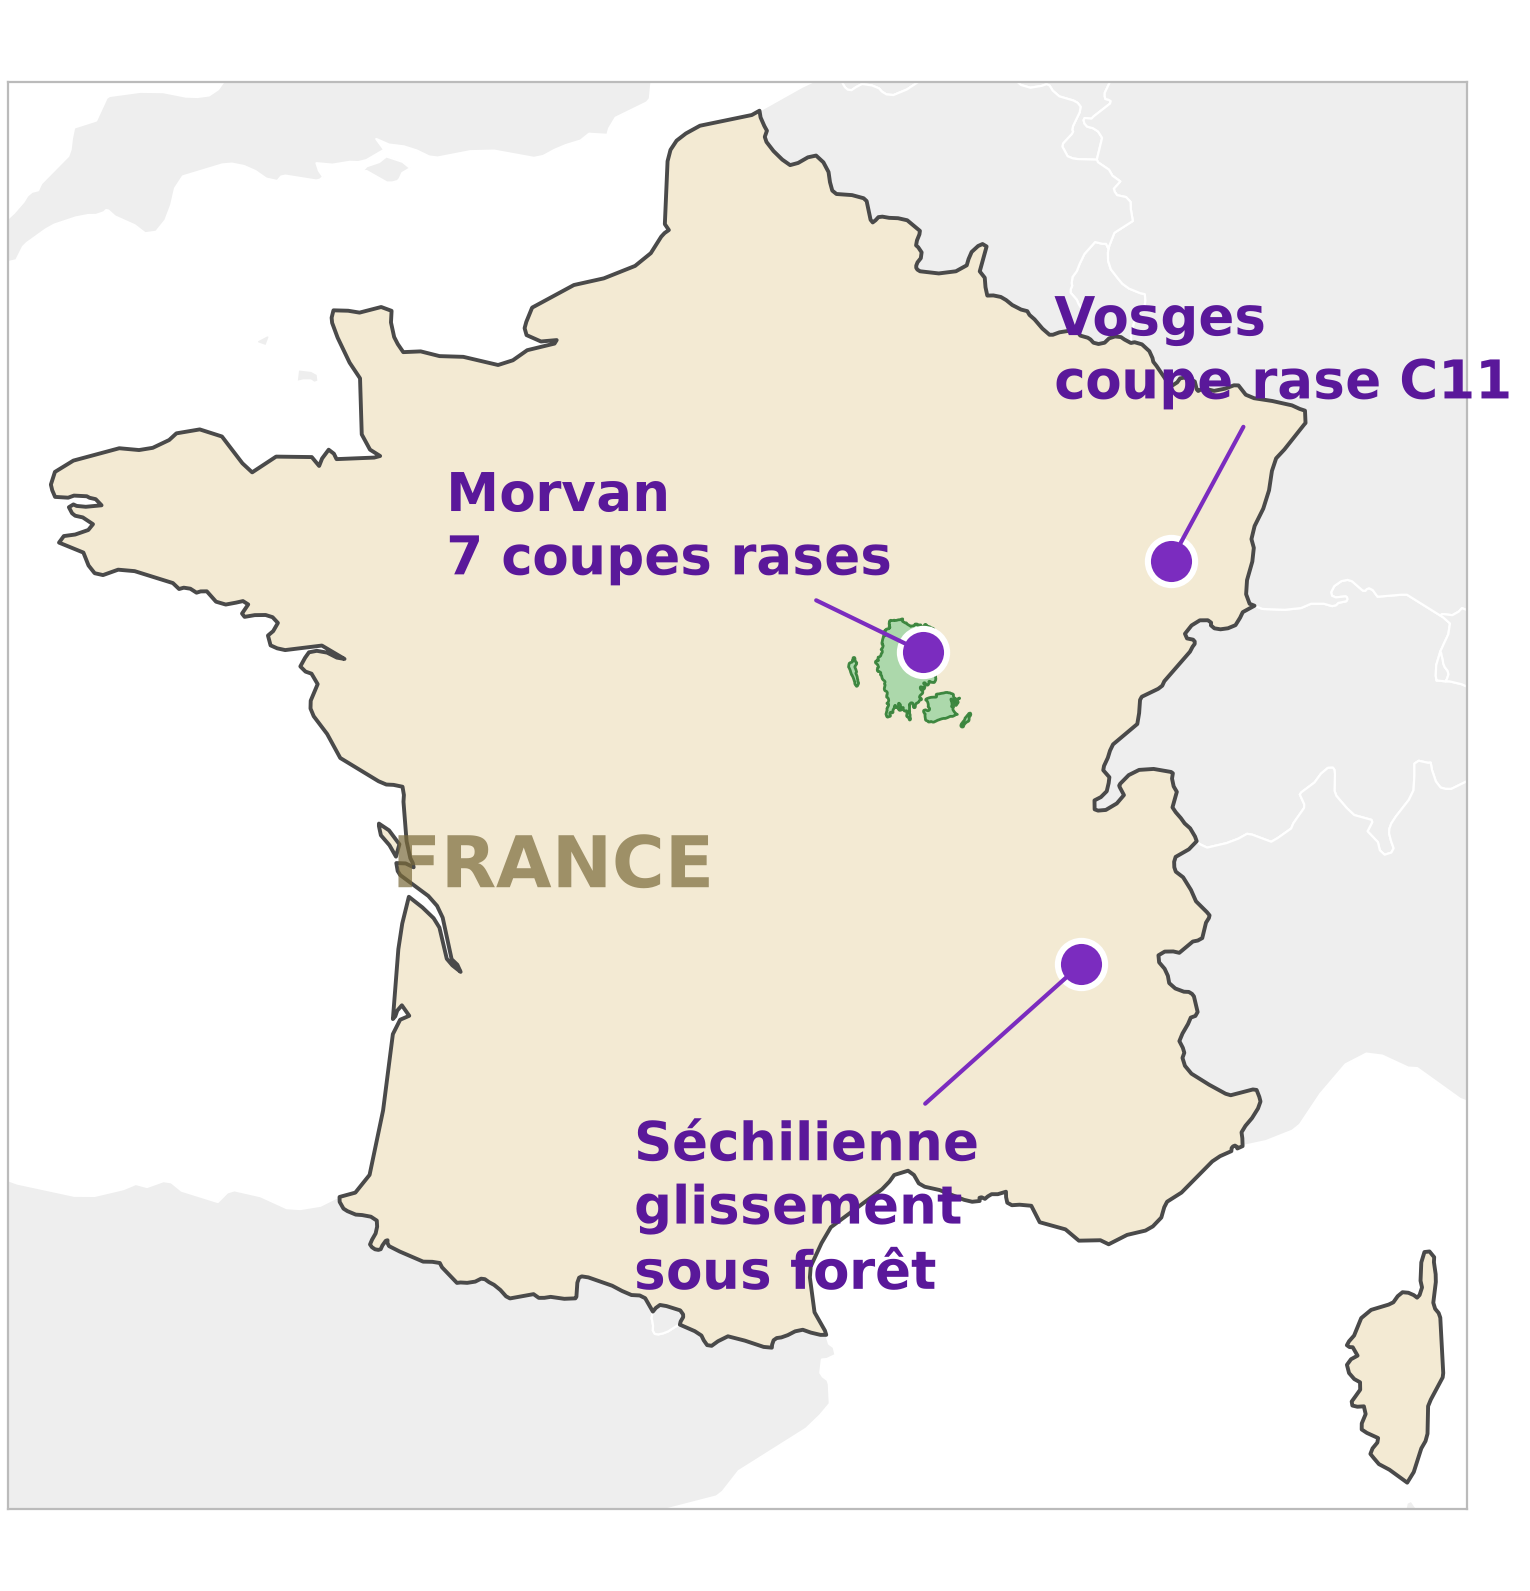
\includegraphics[width=\linewidth]{f0_localisation.png}
\end{minipage}\hfill
\begin{minipage}[c]{0.59\linewidth}
\textbf{Vosges} : une coupe de 2,36 ha réalisée début août 2026 près du Thillot, datée et délimitée avec
Sentinel-2, et sa forêt témoin.\par\vspace{3mm}
\textbf{Morvan} (sylvo-écorégion G23, en vert) : fenêtre de 20 $\times$ 20 km où la méthode du guide de
l'Irstea [3] fournit la référence ; 7 coupes de peuplement fermé photo-interprétées (15,4 ha).\par\vspace{3mm}
\textbf{Séchilienne} (Isère) : versant boisé instable de 168 ha et forêt témoin stable de même exposition.
\end{minipage}
\figcap{Localisation des trois sites (limites Natural Earth).}
\vspace{2mm}
\tabcap{Données (juin -- novembre 2026, toutes en accès libre).}
\begin{center}\small
\begin{tabularx}{\linewidth}{@{}lXXl@{}}
\toprule
Site & \Lb{NISAR, bande L} & \Cb{Sentinel-1, bande C} & Référence \\
\midrule
Vosges & GUNW + GCOV, 3 géométries (A144, A72, D138) & SLC, orbite D139, 13 dates (SNAP) & NDVI Sentinel-2 \\
Morvan & GUNW + GCOV, A173 et D66 & SLC, orbites A59 et D37, 15 dates & guide Irstea \\
Séchilienne & GUNW, A173 (9 paires), D138 (8) & SLC, A161 et D139, mêmes 17 paires & zones sans radar \\
\bottomrule
\end{tabularx}\end{center}
}

\block{3. Méthode}{
\begin{center}\resizebox{0.9\linewidth}{!}{%
\begin{tikzpicture}[font=\normalsize, node distance=9mm and 7mm,
  bx/.style={draw=nuit!70, fill=white, rounded corners=3mm, line width=1mm, align=center, minimum height=24mm},
  fl/.style={-{Latex[length=7mm,width=6mm]}, line width=1.4mm, nuit!70}]
\node[bx, draw=bandeL, fill=bandeL!8, text width=13cm] (n) {\textbf{NISAR GUNW + GCOV}\\ lecture à distance par fenêtre};
\node[bx, draw=bandeC, fill=bandeC!8, text width=13cm, right=of n] (s) {\textbf{Sentinel-1 SLC}\\ cohérence, $\gamma^0$, phase (SNAP)};
\node[bx, text width=12cm, right=of s] (o) {\textbf{Référence}\\ Sentinel-2, guide Irstea, MNT};
\node[bx, text width=40cm, below=14mm of s] (g) {\textbf{Paquet \texttt{nisar\_s1}} : grille commune 20 m, mêmes dates et mêmes paires pour les deux bandes};
\node[bx, fill=accent!12, text width=19cm, below=14mm of g.south west, anchor=north west] (a) {\textbf{Coupes rases}\\ AUC coupe / forêt, IC par bootstrap ;\\ méthode du guide transposée au radar (kappa)};
\node[bx, fill=accent!12, text width=19cm, below=14mm of g.south east, anchor=north east] (b) {\textbf{Glissement}\\ cohérence et consistance de phase\\ du versant, référencées sur le témoin};
\draw[fl] (n.south) -- (n.south|-g.north); \draw[fl] (s.south) -- (s.south|-g.north); \draw[fl] (o.south) -- (o.south|-g.north);
\draw[fl] (a.north|-g.south) -- (a.north); \draw[fl] (b.north|-g.south) -- (b.north);
\end{tikzpicture}}
\end{center}
\figcap{Schéma de la méthode. AUC : aire sous la courbe ROC, probabilité qu'un pixel de coupe et un pixel de forêt
tirés au hasard soient correctement ordonnés (0,5 = indiscernables, 1 = séparation parfaite). Consistance de
phase : module de la moyenne des phases (1 = phase uniforme, 0 = phase aléatoire).}
}

\block{4. Résultats}{
\sous{4.1 Vosges : la cohérence L sépare la coupe dans toutes les géométries}
\fig{f1_vosges.png}
\figcap{AUC de séparation entre la coupe C11 et la forêt témoin, par indicateur et par géométrie ; contour
noir : géométries descendantes, la comparaison à géométrie égale entre les deux bandes.}
\cle{La paire NISAR qui encadre la coupe donne une cohérence de 0,29 sur la coupe contre 0,69 en forêt :
\Lb{AUC 0,995}, même sur 24 jours ; en bande C, la forêt est déjà décorrélée en 12 jours (0,28) et l'AUC
plafonne à \Cb{0,74}. En rétrodiffusion croisée, l'avantage de la bande L dépend de la géométrie : à
géométrie égale (descendante), la bande C fait au moins aussi bien (0,91 contre 0,84).}
}

% ===================================================================== colonne droite
\column{0.5}

\block{4. Résultats (suite)}{
\sous{4.2 Morvan : à géométrie égale, la méthode du guide marche mieux en bande L}
\fig{f2_morvan.png}
\figcap{AUC entre 7 coupes vérifiées et la forêt intacte, avec IC à 95\,\% par bootstrap sur les coupes :
a) géométrie montante ; b) géométrie descendante.}
\vspace{2mm}
\tabcap{Méthode du guide transposée au radar (meilleure combinaison), 7 coupes de référence.}
\begin{center}{\setlength{\tabcolsep}{16pt}
\begin{tabular}{lcccc}
\toprule
 & \Lb{L A173} & \Cb{C A59} & \Lb{L D66} & \Cb{C D37} \\
\midrule
kappa & \Lb{0,41} & \Cb{0,08} & \Lb{0,41} & \Cb{0,16} \\
coupes trouvées & 5 / 7 & 2--3 / 7 & 5 / 7 & 2--3 / 7 \\
\bottomrule
\end{tabular}}\end{center}
En cohérence descendante, la bande L sépare les coupes (\Lb{0,81}) quand la bande C reste au hasard
(\Cb{0,52}). En rétrodiffusion, les AUC sont proches, mais le contraste est plus marqué en L (d de Cohen
1,9--2,1 contre 1,0--1,6), ce qu'exige une méthode à seuil comme celle du guide.

\sous{4.3 Séchilienne : la phase L reste cohérente sous la forêt}
\fig{f3_sechilienne.png}
\figcap{Versant boisé en mouvement, 17 paires à 12 ou 24 jours (26 juin -- 24 octobre 2026) : a) cohérence
médiane ; b) consistance de phase, référencée sur la forêt témoin. Trait noir : médiane des paires.}
La bande C est décorrélée sur tout le versant (cohérence 0,28--0,29, plancher de l'estimateur, alors qu'elle
atteint 0,97--0,99 sur le bâti) et sa phase est aléatoire (\Cb{0,09--0,11}). La phase L reste consistante
(\Lb{0,88--0,92}) : c'est la condition nécessaire pour mesurer un déplacement sous forêt. Aucun déplacement
ne dépasse le bruit en 4 mois ($-$4 à +5 mm), la vitesse attendue étant de l'ordre du cm par an.
}

\block{5. Discussion et conclusions}{
Cette étude compare les bandes L (NISAR) et C (Sentinel-1) sur trois cas forestiers français, avec les
premières données NISAR de 2026. Le message est le même sur les trois sites : \textbf{l'avantage robuste de la
bande L sous la forêt est interférométrique}. À 12 jours, la forêt garde une cohérence de 0,3 à 0,7 en L
contre 0,25 à 0,36 en C, au plancher de l'estimateur, ce qui donne une cohérence qui isole les coupes (AUC \Lb{0,995} dans les Vosges,
\Lb{0,81} dans le Morvan) et une phase exploitable sur un versant boisé (\Lb{0,92} contre \Cb{0,11}). En
rétrodiffusion, l'écart est plus faible et dépend de la géométrie : à géométrie égale, la bande C reste
compétitive, mais le contraste plus fort de la bande L profite aux méthodes à seuil (kappa \Lb{0,41} contre
\Cb{0,08--0,16}). Ces résultats restent limités : une seule saison, quelques coupes, une référence optique
qui conditionne tout (avec la référence automatique, aucune bande ne sépare les coupes). \textbf{Ainsi, en
perspective}, une série NISAR d'au moins un an pour mesurer le glissement, davantage de coupes et une
détection fondée sur la cohérence sont des pistes à explorer, en préparation de la mission \textbf{ROSE-L}.
}
\block{Références}{\footnotesize
\begin{enumerate}[label={[\arabic*]},leftmargin=2.1em,itemsep=2pt]
\item Kellogg \textit{et al.} (2020), \textit{IEEE Aerospace Conf.}, 1--21.
\item Torres \textit{et al.} (2012), \textit{Remote Sens. Environ.} 120, 9--24.
\item Ose \& Deshayes (2015), guide méthodologique, Irstea.
\item Zebker \& Villasenor (1992), \textit{IEEE TGRS} 30, 950--959.
\item Joshi \textit{et al.} (2015), \textit{Environ. Res. Lett.} 10, 034014.
\end{enumerate}
\vspace{3mm}
{\color{gris}\textbf{Données} : NISAR L2 (NASA--ISRO ; produits JPL générés avec \textbf{ISCE3}, ASF DAAC),
Copernicus Sentinel-1 et Sentinel-2 (ESA, UE), IGN (BD Forêt, RGE ALTI).
\textbf{Code} : \texttt{nisar\_s1}, github.com/mamadou-g-diallo/nisar-s1 ; étude :
github.com/mamadou-g-diallo/nisar-s1-forest-france (Apache-2.0).\par}
}
\end{columns}
\end{document}
